\chapter{Euclidean Correlation Functions and Gaussian Perturbation Theory}
\label{ch:euclidean-correlation-functions-gaussian-perturbation}

\section{Spectral Correlators and Euclidean Time}

Let \(\widehat H\) be a self-adjoint Hamiltonian on a Hilbert space
\(\Hilb\). Assume in this section that \(\widehat H\) has a normalized
ground state \(\ket 0\) with energy \(E_0\), and that the example under
discussion admits a complete orthonormal basis \(\{\ket n\}\) of energy
eigenvectors,
\[
  \widehat H\ket n=E_n\ket n,\qquad E_n\ge E_0.
\]
For a self-adjoint coordinate operator \(\widehat q\), define the real-time
Heisenberg operator
\[
  \widehat q(t)
  =
  \exp\left(\frac{\ii}{\hbar}t\widehat H\right)
  \widehat q
  \exp\left(-\frac{\ii}{\hbar}t\widehat H\right),
  \qquad t\in\mathbb R.
\]
The ordered two-point function with the later insertion on the left is
\[
  W(t)=\bra 0\widehat q(t)\widehat q(0)\ket 0 .
\]
Inserting the energy basis gives
\[
\begin{aligned}
  W(t)
  &=
  \sum_n
  \bra 0\widehat q(0)\ket n
  \bra n\widehat q(0)\ket 0\,
  \exp\left[-\frac{\ii}{\hbar}(E_n-E_0)t\right]  \\
  &=
  \sum_n
  \left|\bra n\widehat q(0)\ket 0\right|^2
  \exp\left[-\frac{\ii}{\hbar}(E_n-E_0)t\right].
\end{aligned}
\]
When the matrix elements have the convergence properties needed for this
series or its distributional analogue, the spectrum condition
\(E_n-E_0\ge0\) gives an analytic continuation to the lower half \(t\)-plane.
For \(\tau>0\), define
\[
  G_E(\tau)
  =
  W(-\ii\tau)
  =
  \sum_n
  \left|\bra n\widehat q(0)\ket 0\right|^2
  \exp\left[-\frac{1}{\hbar}(E_n-E_0)\tau\right].
\]
Thus Euclidean time converts the spectral decomposition into a sum of
decaying exponentials. The decay rates are
\[
  \omega_n=\frac{E_n-E_0}{\hbar}.
\]

For \(\tau_1,\ldots,\tau_r\in\mathbb R\), let \(T_E\) denote Euclidean
ordering: operators with larger \(\tau\) are placed to the left. The Euclidean
\(r\)-point function of a single coordinate operator is
\[
  G_E^{(r)}(\tau_1,\ldots,\tau_r)
  =
  \bra 0
  T_E\{\widehat q_E(\tau_1)\cdots\widehat q_E(\tau_r)\}
  \ket 0,
\]
where
\[
  \widehat q_E(\tau)
  =
  \exp\left(\frac{1}{\hbar}\tau\widehat H\right)
  \widehat q
  \exp\left(-\frac{1}{\hbar}\tau\widehat H\right)
\]
is the analytic continuation of \(\widehat q(t)\) to \(t=-\ii\tau\).

It is useful to package the ordered functions by a source. For a smooth
compactly supported function \(J(\tau)\), define
\[
  Z_E[J]
  =
  \bra 0
  T_E
  \exp\left[
    \frac{1}{\hbar}
    \int_{\mathbb R}J(\tau)\widehat q_E(\tau)\,\dd\tau
  \right]
  \ket 0 .
\]
The correlation functions are obtained by
\[
  G_E^{(r)}(\tau_1,\ldots,\tau_r)
  =
  \left.
  \hbar^r
  \frac{\delta}{\delta J(\tau_1)}
  \cdots
  \frac{\delta}{\delta J(\tau_r)}
  Z_E[J]
  \right|_{J=0}.
\]

\section{Wick Rotation of the Path Integral}

Consider a Lagrangian of the form
\[
  L(q,\dot q)
  =
  \frac12G_{ab}(q)\dot q^a\dot q^b-V(q),
\]
where \(G_{ab}(q)\) is positive definite. Under the analytic continuation
\[
  t=-\ii\tau,\qquad
  \dot q^a=\frac{\dd q^a}{\dd t}
  =
  \ii\,\frac{\dd q^a}{\dd\tau},
\]
define the Euclidean Lagrangian
\[
  L_E(q,q')
  =
  -L(q,\ii q'),
  \qquad q'^a=\frac{\dd q^a}{\dd\tau}.
\]
For the displayed \(L\), this gives
\[
  L_E(q,q')
  =
  \frac12G_{ab}(q)q'^aq'^b+V(q).
\]
The Lorentzian phase transforms as
\[
  \exp\left[
    \frac{\ii}{\hbar}\int L(q,\dot q)\,\dd t
  \right]
  \longmapsto
  \exp\left[
    -\frac{1}{\hbar}\int L_E(q,q')\,\dd\tau
  \right].
\]

Let \(\ket\psi\in\Hilb\) satisfy \(\braket{0}{\psi}\ne0\), and assume for this
paragraph that the ground state is separated from the rest of the spectrum by
a gap. Then
\[
  \frac{\exp[-T(\widehat H-E_0)/\hbar]\ket\psi}
       {\left\|\exp[-T(\widehat H-E_0)/\hbar]\ket\psi\right\|}
  \longrightarrow
  \ket 0
\]
up to phase as \(T\to\infty\). For \(0<\tau_1<\cdots<\tau_r<T\), the
Euclidean correlation function is the long-time limit of matrix elements of
\(\exp(-\tau\widehat H/\hbar)\) with insertions at the specified Euclidean
times. In the Lagrangian path-integral notation this is expressed as
\[
  \bra 0T_E\{\widehat q_E(\tau_1)\cdots\widehat q_E(\tau_r)\}\ket 0
  =
  \lim_{T\to\infty}
  \frac{
    \int [Dq]\,\exp[-S_E[q]/\hbar]\,
    q(\tau_1)\cdots q(\tau_r)
  }{
    \int [Dq]\,\exp[-S_E[q]/\hbar]
  },
\]
where the symbol \([Dq]\) denotes a specified regulator and limiting
procedure, and
\[
  S_E[q]=\int_{-T}^{T}L_E(q,q')\,\dd\tau.
\]

\begin{center}
\begin{tikzpicture}[>=Stealth,scale=0.95]
  \draw[->] (-3.2,0) -- (3.35,0) node[right] {$\operatorname{Re}t$};
  \draw[->] (0,-2.15) -- (0,2.15) node[above] {$-\operatorname{Im}t=\tau$};
  \draw[blue!70!black,line width=1pt,->] (0,0) -- (2.05,0);
  \node[blue!70!black,below] at (1.1,0) {real time};
  \draw[green!45!black,line width=1pt,->] (0,0) -- (0,1.75);
  \node[green!45!black,anchor=west] at (0.18,1.55) {Euclidean time};
  \draw[orange!80!black,line width=0.9pt,->]
    (1.45,0) arc[start angle=0,end angle=90,radius=1.45];
  \node[orange!80!black] at (1.28,0.82) {$t=-\ii\tau$};
  \fill (0,0) circle (1.8pt);
\end{tikzpicture}
\end{center}

\begin{center}
\begin{tikzpicture}[>=Stealth,scale=0.95]
  \draw[->] (-3.2,0) -- (3.35,0) node[right] {$\tau$};
  \draw[line width=0.8pt,blue!65!black] (-2.6,0) -- (2.6,0);
  \foreach \x/\lab in {-2.6/{-T},0/{0},1.15/{\tau},2.6/{T}} {
    \fill (\x,0) circle (2pt);
    \node[below=3pt] at (\x,0) {$\lab$};
  }
  \draw[decorate,decoration={brace,amplitude=4pt}]
    (-2.6,0.35) -- node[midway,above=5pt] {\scriptsize projection} (0,0.35);
  \draw[decorate,decoration={brace,amplitude=4pt,mirror}]
    (0,-0.42) -- node[midway,below=5pt] {\scriptsize ordered insertions} (1.15,-0.42);
  \draw[decorate,decoration={brace,amplitude=4pt}]
    (1.15,0.35) -- node[midway,above=5pt] {\scriptsize projection} (2.6,0.35);
\end{tikzpicture}
\end{center}

\section{The Harmonic Oscillator}

Let
\[
  \widehat H=\frac12(\widehat p^2+\omega^2\widehat q^2),
  \qquad
  L(q,\dot q)=\frac12\dot q^2-\frac12\omega^2q^2,
\]
with \(\omega>0\). The Euclidean action on the interval \([-T,T]\) is
\[
  S_E[q]
  =
  \frac12\int_{-T}^{T}
  \left[
    (q')^2+\omega^2q^2
  \right]\dd\tau .
\]
Impose Dirichlet boundary conditions \(q(-T)=q(T)=0\) and expand
\[
  q(\tau)=\sum_{n=1}^{\infty}q_nf_n(\tau),
  \qquad
  f_n(\tau)=\frac{1}{\sqrt T}
  \sin\frac{n\pi(\tau+T)}{2T}.
\]
The functions \(f_n\) obey
\[
  \int_{-T}^{T}f_n(\tau)f_m(\tau)\,\dd\tau=\delta_{nm},
  \qquad
  -\frac{\dd^2}{\dd\tau^2}f_n
  =
  \left(\frac{n\pi}{2T}\right)^2f_n .
\]
Consequently
\[
  S_E[q]
  =
  \frac12\sum_{n=1}^{\infty}
  \left[
    \left(\frac{n\pi}{2T}\right)^2+\omega^2
  \right]q_n^2 .
\]

\begin{center}
\begin{tikzpicture}[>=Stealth,scale=0.95]
  \draw[->] (-3.2,0) -- (3.4,0) node[right] {$\tau$};
  \draw[->] (0,-1.15) -- (0,1.55) node[above] {$q(\tau)$};
  \draw[purple!80!black,line width=1pt]
    (-2.55,0)
    .. controls (-2.05,0.75) and (-1.38,0.95) .. (-0.92,0.05)
    .. controls (-0.52,-0.82) and (-0.12,-0.74) .. (0.25,0.22)
    .. controls (0.74,1.18) and (1.65,0.98) .. (2.55,0);
  \fill (-2.55,0) circle (2pt) node[below] {$-T$};
  \fill (2.55,0) circle (2pt) node[below] {$T$};
  \node[below] at (0,-1.0) {$q(-T)=q(T)=0$};
\end{tikzpicture}
\end{center}

Define the normalized finite-\(T\) expectation value by
\[
  \langle F\rangle_T
  =
  \frac{
    \int\prod_{n=1}^{\infty}\dd q_n\,
    \exp[-S_E[q]/\hbar]\,F
  }{
    \int\prod_{n=1}^{\infty}\dd q_n\,
    \exp[-S_E[q]/\hbar]
  },
\]
with the understanding that a finite mode cutoff is used before the limiting
operation. The independent Gaussian integrals give
\[
  \langle q_nq_m\rangle_T
  =
  \delta_{nm}\,
  \frac{\hbar}{
    \left(\frac{n\pi}{2T}\right)^2+\omega^2
  }.
\]
Therefore
\[
  \langle q(\tau_1)q(\tau_2)\rangle_T
  =
  \sum_{n=1}^{\infty}
  \frac{\hbar\,f_n(\tau_1)f_n(\tau_2)}
       {\left(\frac{n\pi}{2T}\right)^2+\omega^2}.
\]
Taking \(T\to\infty\) gives
\[
  \langle q(\tau_1)q(\tau_2)\rangle
  =
  \hbar
  \int_{-\infty}^{\infty}\frac{\dd k}{2\pi}\,
  \frac{\ee^{\ii k(\tau_1-\tau_2)}}{k^2+\omega^2}.
\]
The remaining integral is evaluated by residues. For \(\tau>0\), close the
contour in the upper half-plane:
\[
  \int_{-\infty}^{\infty}
  \frac{\ee^{\ii k\tau}}{k^2+\omega^2}\,\dd k
  =
  \frac{\pi}{\omega}\ee^{-\omega\tau}.
\]
For \(\tau<0\), close the contour in the lower half-plane and obtain
\(\pi\omega^{-1}\ee^{\omega\tau}\).

\begin{center}
\begin{tikzpicture}[>=Stealth,scale=0.98]
  \draw[line width=0.6pt] (-2.65,-1.75) rectangle (2.65,1.75);
  \draw[->] (-2.35,0) -- (2.35,0) node[right] {$\operatorname{Re}k$};
  \draw[->] (0,-1.45) -- (0,1.45) node[above] {$\operatorname{Im}k$};
  \draw[green!45!black,line width=1pt,->]
    (-2.0,0) arc[start angle=180,end angle=25,radius=2.0];
  \draw[green!45!black,line width=1pt]
    (1.81,0.84) arc[start angle=25,end angle=0,radius=2.0];
  \node[red!80!black] at (0,0.95) {$\times$};
  \node[right=2pt] at (0,0.95) {$\ii\omega$};
  \node[red!80!black] at (0,-0.95) {$\times$};
  \node[right=2pt] at (0,-0.95) {$-\ii\omega$};
  \node[align=center] at (0,-1.95) {upper contour for \(\tau>0\)};
\end{tikzpicture}
\end{center}

The Euclidean two-point function of the harmonic oscillator is
\[
  \boxed{
  \langle q(\tau_1)q(\tau_2)\rangle
  =
  \frac{\hbar}{2\omega}
  \ee^{-\omega|\tau_1-\tau_2|}
  }.
\]
This agrees with the spectral expression, since the first operator
\(\widehat q\) connects the ground state of the harmonic oscillator to the
first excited state.

\section{Gaussian Integrals and Wick Pairings}

For the remainder of the chapter set \(\hbar=1\), unless \(\hbar\) is
displayed explicitly. Let \(A\) be a real symmetric positive-definite \(N\times N\)
matrix, and let \(J\in\mathbb R^N\). Define
\[
  Z_A[J]
  =
  \int_{\mathbb R^N}\dd^Nq\,
  \exp\left(
    -\frac12q_iA_{ij}q_j+J_iq_i
  \right),
\]
where repeated finite indices are summed. Completing the square gives
\[
  Z_A[J]
  =
  (2\pi)^{N/2}(\det A)^{-1/2}
  \exp\left(
    \frac12J_i(A^{-1})_{ij}J_j
  \right).
\]
The normalized Gaussian expectation of a function \(F(q)\) is
\[
  \langle F(q)\rangle_A
  =
  \frac{1}{Z_A[0]}
  \int_{\mathbb R^N}\dd^Nq\,
  \exp\left(-\frac12q_iA_{ij}q_j\right)F(q).
\]
Differentiating with respect to \(J\) gives
\[
  \langle F(q)\rangle_A
  =
  \left.
  F\left(\frac{\partial}{\partial J}\right)
  \frac{Z_A[J]}{Z_A[0]}
  \right|_{J=0}.
\]
In particular,
\[
  \langle q_i\rangle_A=0,\qquad
  \langle q_iq_j\rangle_A=(A^{-1})_{ij}.
\]
For four variables,
\[
\begin{aligned}
  \langle q_iq_jq_kq_\ell\rangle_A
  &=
  (A^{-1})_{ij}(A^{-1})_{k\ell}
  +(A^{-1})_{ik}(A^{-1})_{j\ell}  \\
  &\quad
  +(A^{-1})_{i\ell}(A^{-1})_{jk}.
\end{aligned}
\]

\begin{center}
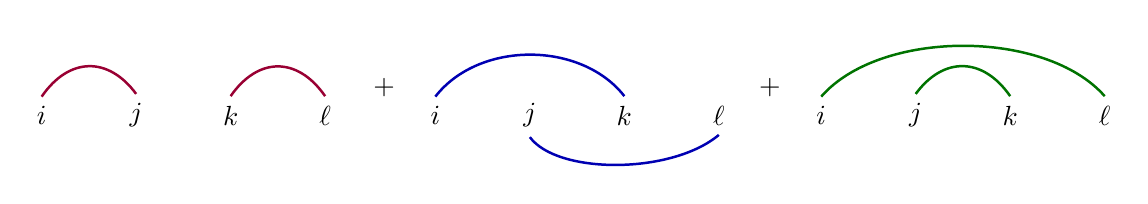
\begin{tikzpicture}[scale=1.0]
  \node (i) at (0,0) {$i$};
  \node (j) at (1.2,0) {$j$};
  \node (k) at (2.4,0) {$k$};
  \node (l) at (3.6,0) {$\ell$};
  \draw[purple!80!black,line width=0.9pt]
    (i.north) .. controls (0.35,0.75) and (0.85,0.75) .. (j.north);
  \draw[purple!80!black,line width=0.9pt]
    (k.north) .. controls (2.75,0.75) and (3.25,0.75) .. (l.north);
  \node at (4.35,0.35) {$+$};
  \node (i2) at (5.0,0) {$i$};
  \node (j2) at (6.2,0) {$j$};
  \node (k2) at (7.4,0) {$k$};
  \node (l2) at (8.6,0) {$\ell$};
  \draw[blue!70!black,line width=0.9pt]
    (i2.north) .. controls (5.55,0.95) and (6.85,0.95) .. (k2.north);
  \draw[blue!70!black,line width=0.9pt]
    (j2.south) .. controls (6.55,-0.75) and (8.0,-0.75) .. (l2.south);
  \node at (9.25,0.35) {$+$};
  \node (i3) at (9.9,0) {$i$};
  \node (j3) at (11.1,0) {$j$};
  \node (k3) at (12.3,0) {$k$};
  \node (l3) at (13.5,0) {$\ell$};
  \draw[green!45!black,line width=0.9pt]
    (i3.north) .. controls (10.65,1.1) and (12.75,1.1) .. (l3.north);
  \draw[green!45!black,line width=0.9pt]
    (j3.north) .. controls (11.45,0.75) and (11.95,0.75) .. (k3.north);
\end{tikzpicture}
\end{center}

A Wick contraction is an assigned pairing of two labels with value
\[
  (q_iq_j)_{\mathrm{contr}}=(A^{-1})_{ij}.
\]
Wick's theorem says that the Gaussian expectation of \(2r\) variables is the
sum over all complete pairings, with one covariance factor for each pair:
\[
  \langle q_{i_1}\cdots q_{i_{2r}}\rangle_A
  =
  \sum_{\text{complete pairings }P}
  \prod_{(a,b)\in P}(A^{-1})_{i_ai_b}.
\]
Gaussian expectations of an odd number of variables vanish.

\section{Gaussian Functional Integrals}

Let \(A\) be the positive operator
\[
  A=-\frac{\dd^2}{\dd\tau^2}+\omega^2
\]
on a function space with boundary conditions for which \(A\) is invertible.
The Green function \(G(\tau,\tau')\) is the integral kernel of \(A^{-1}\):
\[
  (A^{-1}f)(\tau)
  =
  \int G(\tau,\tau')f(\tau')\,\dd\tau',
\]
and therefore satisfies
\[
  \left(
    -\frac{\dd^2}{\dd\tau^2}+\omega^2
  \right)G(\tau,\tau')
  =
  \delta(\tau-\tau').
\]
With the inner product
\[
  (f,g)=\int f(\tau)g(\tau)\,\dd\tau,
\]
the Gaussian Euclidean action is
\[
  S_0[q]=\frac12(q,Aq).
\]
The source-dependent Gaussian functional integral is defined by a regulator,
for instance a finite-mode cutoff, and has the finite-dimensional form in the
cutoff variables. Its continuum notation is
\[
  Z_0[J]
  =
  \int[Dq]\,
  \exp\left[
    -\frac12(q,Aq)+(J,q)
  \right].
\]
The ratio independent of normalization is
\[
  \frac{Z_0[J]}{Z_0[0]}
  =
  \exp\left[
    \frac12\int J(\tau)G(\tau,\tau')J(\tau')\,
    \dd\tau\,\dd\tau'
  \right].
\]
Consequently
\[
  \langle q(\tau_1)q(\tau_2)\rangle_0
  =
  G(\tau_1,\tau_2).
\]

On the infinite Euclidean line, write
\[
  q(\tau)=
  \int_{-\infty}^{\infty}\frac{\dd k}{2\pi}\,
  \widetilde q(k)\ee^{\ii k\tau},
  \qquad
  \widetilde q(k)^*=\widetilde q(-k).
\]
Then
\[
  S_0[q]
  =
  \frac12
  \int_{-\infty}^{\infty}\frac{\dd k}{2\pi}\,
  \widetilde q(-k)(k^2+\omega^2)\widetilde q(k),
\]
and
\[
  \langle \widetilde q(k_1)\widetilde q(k_2)\rangle_0
  =
  \frac{2\pi\delta(k_1+k_2)}{k_1^2+\omega^2}.
\]
Thus
\[
  G(\tau,\tau')
  =
  \int_{-\infty}^{\infty}
  \frac{\dd k}{2\pi}\,
  \frac{\ee^{\ii k(\tau-\tau')}}{k^2+\omega^2}
  =
  \frac{1}{2\omega}\ee^{-\omega|\tau-\tau'|}.
\]

\section{The Anharmonic Oscillator}

Set \(\omega=1\) in this section. The anharmonic oscillator is defined by
\[
  \widehat H
  =
  \frac12\widehat p^2+\frac12\widehat q^2+\frac{g}{4!}\widehat q^4.
\]
The Euclidean Lagrangian is
\[
  L_E(q,q')
  =
  \frac12(q')^2+\frac12q^2+\frac{g}{4!}q^4.
\]
Let
\[
  S_0[q]=\int\left[\frac12(q')^2+\frac12q^2\right]\dd\tau,
  \qquad
  S_{\mathrm{int}}[q]=\frac{g}{4!}\int q(\tau)^4\,\dd\tau .
\]
At finite cutoff, perturbation theory is the expansion of
\(\exp[-S_{\mathrm{int}}]\) inside a finite-dimensional Gaussian integral.
For the partition function,
\[
  Z_g=\int[Dq]\,\exp[-S_0[q]-S_{\mathrm{int}}[q]],
\]
one obtains
\[
  \frac{Z_g}{Z_0}
  =
  \sum_{n=0}^{\infty}
  \frac{1}{n!}
  \left(-\frac{g}{4!}\right)^n
  \int \dd\tau_1\cdots\dd\tau_n\,
  \left\langle
    q(\tau_1)^4\cdots q(\tau_n)^4
  \right\rangle_0 .
\]
Here \(Z_0\) is the Gaussian partition function and
\(\langle\cdots\rangle_0\) is evaluated with
\[
  G_0(\tau,\tau')=\frac12\ee^{-|\tau-\tau'|}.
\]

At first order in \(g\),
\[
  -\frac{g}{4!}\int\dd\tau\,\langle q(\tau)^4\rangle_0
  =
  -\frac{g}{8}\int\dd\tau\,G_0(\tau,\tau)^2.
\]
The factor \(3\) in \(\langle q^4\rangle_0=3G_0(\tau,\tau)^2\) is the number
of pairings of four fields at the vertex.

\begin{center}
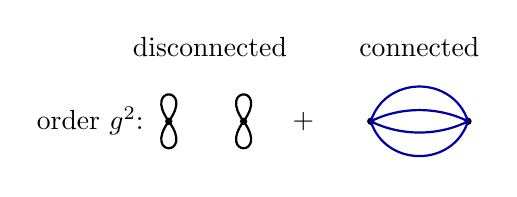
\begin{tikzpicture}[scale=0.95]
  \node at (-1.2,0) {order \(g^2\):};
  \node at (0.4,1.0) {disconnected};
  \foreach \x in {-0.15,0.85} {
    \draw[thick] (\x,0) .. controls (\x-0.35,0.48) and (\x+0.35,0.48) .. (\x,0);
    \draw[thick] (\x,0) .. controls (\x-0.35,-0.48) and (\x+0.35,-0.48) .. (\x,0);
    \fill (\x,0) circle (1.4pt);
  }
  \node at (1.65,0) {$+$};
  \node at (3.2,1.0) {connected};
  \foreach \x in {2.55,3.85} {
    \fill (\x,0) circle (1.4pt);
  }
  \draw[thick,blue!65!black]
    (2.55,0) .. controls (2.75,0.62) and (3.65,0.62) .. (3.85,0);
  \draw[thick,blue!65!black]
    (2.55,0) .. controls (2.75,-0.62) and (3.65,-0.62) .. (3.85,0);
  \draw[thick,blue!65!black]
    (2.55,0) .. controls (2.95,0.2) and (3.45,0.2) .. (3.85,0);
  \draw[thick,blue!65!black]
    (2.55,0) .. controls (2.95,-0.2) and (3.45,-0.2) .. (3.85,0);
\end{tikzpicture}
\end{center}

Let \(G^{(\ell)}\) be the sum of connected vacuum Wick contractions involving
\(\ell\) interaction vertices, including the coupling factors and integration
over the \(\ell\) vertex positions. If \(m_\ell\) is the number of connected
components of size \(\ell\), then
\[
  \sum_{\ell\ge1}\ell\,m_\ell=n.
\]
The number of ways to partition \(n\) labelled vertices into this pattern is
\[
  \frac{n!}{\prod_{\ell\ge1}(\ell!)^{m_\ell}m_\ell!}.
\]
Summing over all patterns gives the linked-cluster formula
\[
  \frac{Z_g}{Z_0}
  =
  \exp\left[
    \sum_{\ell\ge1}\frac{1}{\ell!}G^{(\ell)}
  \right].
\]
Equivalently, \(\log Z_g\) is the sum of connected vacuum diagrams.

On a long interval of Euclidean length \(T_{\mathrm{tot}}\),
\[
  Z_g\sim \exp[-E_0(g)T_{\mathrm{tot}}],
\]
up to endpoint factors. Hence
\[
  E_0(g)
  =
  -\lim_{T_{\mathrm{tot}}\to\infty}
  \frac{1}{T_{\mathrm{tot}}}\log Z_g.
\]
The first correction is
\[
  \Delta E_0
  =
  \frac{g}{8}G_0(0)^2+O(g^2)
  =
  \frac{g}{32}+O(g^2),
\]
in agreement with first-order Hamiltonian perturbation theory:
\[
  \bra{\psi_0}\frac{g}{4!}\widehat q^4\ket{\psi_0}
  =
  \frac{g}{4!}\,3\left(\frac12\right)^2
  =
  \frac{g}{32}.
\]

\section{Connected Two-Point Functions and Self-Energy}

The normalized Euclidean two-point function is
\[
  G(\tau)
  =
  \langle q(\tau)q(0)\rangle_g
  =
  \frac{1}{Z_g}
  \int[Dq]\,\ee^{-S_0[q]-S_{\mathrm{int}}[q]}\,q(\tau)q(0).
\]
In the perturbative expansion, every Wick contraction splits uniquely into
the connected component containing the two external insertions and a product
of vacuum components. The sum of the vacuum components is \(Z_g\), and is
cancelled by the normalization. Thus \(G(\tau)\) is the sum of connected
two-point diagrams.

\begin{center}
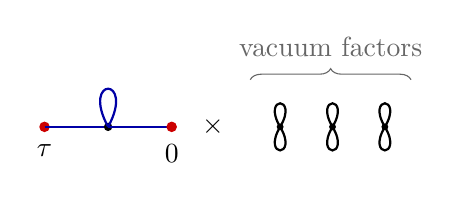
\begin{tikzpicture}[scale=0.95]
  \fill[red!80!black] (0,0) circle (2pt);
  \node[below=3pt] at (0,0) {$\tau$};
  \draw[thick,blue!65!black] (0,0) -- (0.85,0);
  \fill (0.85,0) circle (1.6pt);
  \draw[thick,blue!65!black]
    (0.85,0) .. controls (0.48,0.68) and (1.22,0.68) .. (0.85,0);
  \draw[thick,blue!65!black] (0.85,0) -- (1.7,0);
  \fill[red!80!black] (1.7,0) circle (2pt);
  \node[below=3pt] at (1.7,0) {$0$};
  \node at (2.25,0) {$\times$};
  \draw[decorate,decoration={brace,amplitude=4pt},gray!80!black]
    (2.75,0.63) -- node[midway,above=5pt] {vacuum factors} (4.9,0.63);
  \foreach \x in {3.15,3.85,4.55} {
    \draw[thick] (\x,0) .. controls (\x-0.25,0.42) and (\x+0.25,0.42) .. (\x,0);
    \draw[thick] (\x,0) .. controls (\x-0.25,-0.42) and (\x+0.25,-0.42) .. (\x,0);
    \fill (\x,0) circle (1.3pt);
  }
\end{tikzpicture}
\end{center}

At zeroth order,
\[
  G_0(\tau)=\frac12\ee^{-|\tau|}
  =
  \int_{-\infty}^{\infty}\frac{\dd k}{2\pi}\,
  \frac{\ee^{\ii k\tau}}{k^2+1}.
\]
At order \(g\), the connected tadpole correction is
\[
  -\frac{g}{2}
  \int \dd\tau'\,
  G_0(\tau-\tau')G_0(\tau')G_0(0).
\]
In momentum space this becomes
\[
  -\frac{g}{4}
  \int_{-\infty}^{\infty}\frac{\dd k}{2\pi}\,
  \frac{\ee^{\ii k\tau}}{(k^2+1)^2}.
\]

A connected two-point diagram is one-particle-irreducible, abbreviated
\(1\mathrm{PI}\), when it remains connected after cutting any one internal
propagator. In this chapter the term is graph-theoretic and refers to
Euclidean Green-function diagrams. Let \(\Sigma(k)\) be the sum of amputated
\(1\mathrm{PI}\) two-point insertions in momentum space. Then the full
two-point function is the geometric series
\[
  \widetilde G(k)
  =
  \widetilde G_0(k)
  \sum_{r=0}^{\infty}
  \bigl(\widetilde G_0(k)\Sigma(k)\bigr)^r
  =
  \frac{1}{k^2+1-\Sigma(k)},
  \qquad
  \widetilde G_0(k)=\frac{1}{k^2+1}.
\]

\begin{center}
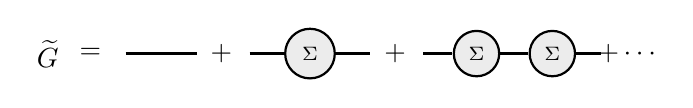
\begin{tikzpicture}[scale=0.9]
  \node at (-0.55,0) {$\widetilde G$};
  \node at (0.05,0) {$=$};
  \draw[thick] (0.55,0) -- (1.55,0);
  \node at (1.9,0) {$+$};
  \draw[thick] (2.3,0) -- (2.8,0);
  \draw[thick,fill=gray!15] (3.15,0) circle (0.35);
  \node at (3.15,0) {\scriptsize \(\Sigma\)};
  \draw[thick] (3.5,0) -- (4.0,0);
  \node at (4.35,0) {$+$};
  \draw[thick] (4.75,0) -- (5.15,0);
  \draw[thick,fill=gray!15] (5.5,0) circle (0.32);
  \node at (5.5,0) {\scriptsize \(\Sigma\)};
  \draw[thick] (5.82,0) -- (6.22,0);
  \draw[thick,fill=gray!15] (6.57,0) circle (0.32);
  \node at (6.57,0) {\scriptsize \(\Sigma\)};
  \draw[thick] (6.89,0) -- (7.25,0);
  \node at (7.62,0) {$+\cdots$};
\end{tikzpicture}
\end{center}

For the anharmonic oscillator,
\[
  \Sigma(k)
  =
  -\frac{g}{4}
  +
  \frac{g^2}{8}
  \left(
    \frac14+\frac{1}{k^2+9}
  \right)
  +O(g^3).
\]
The spectral expansion says that for \(\tau>0\),
\[
  G(\tau)
  =
  \sum_n
  \left|\bra n\widehat q\ket 0\right|^2
  \ee^{-(E_n-E_0)\tau}.
\]
The Fourier representation
\[
  G(\tau)
  =
  \int_{-\infty}^{\infty}\frac{\dd k}{2\pi}\,
  \widetilde G(k)\ee^{\ii k\tau}
\]
is evaluated by closing the contour in the upper half-plane. If
\(\widetilde G(k)\) has simple poles at \(k=\ii\omega_n\), then
\[
  G(\tau)
  =
  \ii\sum_n
  \operatorname*{Res}_{k=\ii\omega_n}\widetilde G(k)\,
  \ee^{-\omega_n\tau}.
\]
Thus the pole positions encode the energy gaps \(\omega_n=E_n-E_0\) in the
\(\hbar=1\) convention. The pole near \(k=\ii\) gives
\[
  E_1-E_0
  =
  1+\frac{g}{8}-\frac{g^2}{32}+O(g^3).
\]

\section{Derivative Interactions, Regulators, and Counterterms}

Consider the Lagrangian
\[
  L(q,\dot q)
  =
  \frac12\dot q^2-\frac12q^2-\frac{g}{8}q^2\dot q^2 .
\]
The canonical momentum is
\[
  p=\frac{\partial L}{\partial\dot q}
  =
  \dot q\left(1-\frac{g}{4}q^2\right),
\]
and the corresponding Hamiltonian function is
\[
  H(q,p)
  =
  \frac12\left(1-\frac{g}{4}q^2\right)^{-1}p^2
  +\frac12q^2.
\]
The Euclidean Lagrangian is
\[
  L_E(q,q')
  =
  \frac12(q')^2+\frac12q^2-\frac{g}{8}q^2(q')^2 .
\]
Using
\[
  q^2(q')^2
  =
  \frac13\frac{\dd}{\dd\tau}(q^3q')
  -\frac13q^3q'',
\]
the interaction may also be represented, up to endpoint terms, by
\[
  \frac{g}{24}q^3q''.
\]

At first order in \(g\), the two-point function contains contractions in
which derivatives act on propagators at coincident points. A representative
term is
\[
  \frac{g}{4}\int\dd\tau'\,
  G_0(\tau-\tau')G_0(\tau')\,
  \bigl[-\partial_{\tau'}^2G_0(\tau'-\tau')\bigr].
\]
In momentum space this contains
\[
  \int\frac{\dd k'}{2\pi}\frac{k'^2}{k'^2+1},
\]
which depends on the high-frequency definition of the path integral.

\begin{center}
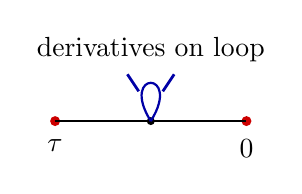
\begin{tikzpicture}[scale=0.9]
  \coordinate (a) at (0,0);
  \coordinate (b) at (1.35,0);
  \coordinate (c) at (2.7,0);
  \fill[red!80!black] (a) circle (2pt);
  \node[below=3pt] at (a) {$\tau$};
  \fill[red!80!black] (c) circle (2pt);
  \node[below=3pt] at (c) {$0$};
  \fill (b) circle (1.6pt);
  \draw[thick] (a) -- (b) -- (c);
  \draw[thick,blue!65!black]
    (b) .. controls (0.9,0.72) and (1.8,0.72) .. (b);
  \draw[blue!65!black,line width=1pt] (1.18,0.42) -- (1.02,0.66);
  \draw[blue!65!black,line width=1pt] (1.52,0.42) -- (1.68,0.66);
  \node[above=18pt] at (b) {derivatives on loop};
\end{tikzpicture}
\end{center}

Define a frequency cutoff by
\[
  q(\tau)
  =
  \int_{|k|<\Lambda}\frac{\dd k}{2\pi}\,
  \widetilde q(k)\ee^{\ii k\tau},
  \qquad
  [Dq]_\Lambda=\prod_{|k|<\Lambda}\dd \widetilde q(k),
\]
with the real-field condition \(\widetilde q(k)^*=\widetilde q(-k)\). After
restoring \(\hbar\), the first-order self-energy has the form
\[
  \Sigma_\Lambda(k)
  =
  \frac{\hbar g}{4}
  \left(
    \frac{\Lambda}{\pi}
    +\frac{k^2}{2}
    -\frac12
    +O(\Lambda^{-1})
  \right)
  +O(\hbar^2g^2).
\]
A local Euclidean counterterm
\[
  \Delta L_E=C\,g\,\hbar\,\frac{q^2}{2}
\]
adds \(-Cg\hbar\) to \(\Sigma_\Lambda(k)\), so that
\[
  \Sigma_\Lambda(k)
  =
  \hbar g
  \left(
    \frac{k^2}{8}
    +\frac{\Lambda}{4\pi}
    -\frac18
    -C
    +O(\Lambda^{-1})
  \right)
  +O(g^2).
\]
Choosing
\[
  C=\frac{\Lambda}{4\pi}+C_{\mathrm{fin}}
\]
defines a finite limiting two-point function as \(\Lambda\to\infty\). The
finite constant \(C_{\mathrm{fin}}\) is part of the quantum definition of the
Hamiltonian represented by this regulated Lagrangian path integral.

The structural statement carried forward to field theory is this: a path
integral with interactions is a regulated construction of Green functions,
and local counterterms are part of the data specifying the regulated
construction and its limiting prescription. The next chapter replaces the
single coordinate \(q(\tau)\) by fields \(\phi(x)\) and imposes relativistic
covariance and locality on the resulting Green functions.
